
\section{Large Scale Distributed Deep Networks}
\indent\setlength{\parindent}{1em} 
Начнем изучение темы распределённого обучения моделей со статьи “Large Scale Distributed Deep Networks” \cite{beginning} , в которой делается большой шаг в сторону распределенного обучения нейронных сетей. 

\indent\setlength{\parindent}{1em} 
Нейронная сеть состоит из нескольких слоев нейронов и синапсов, связей между нейронами. Каждый нейрон принимает на вход какие-то небольшие данные, производит над ними работу и передает полученный результат по синапсу следующему нейрону. У каждого синапса есть вес, который влияет на то, какой вклад внесет результат вычислений одного нейрона на результат вычислений следующего. 
\begin{figure}[h]%current location
	\centering
	\scalebox{0.4}{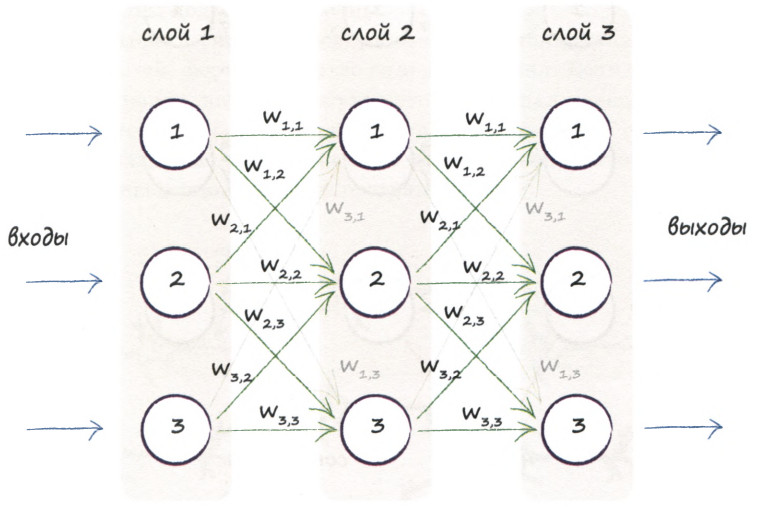
\includegraphics{Parts/images/neural_network.jpg}}
	\caption{Визуализация нейронной сети}
	\label{framework} %framework,fig1
\end{figure}

\indent\setlength{\parindent}{1em} 
Веса синапсов - это одни из параметров нейронной сети и в задачу обучения сети входит подбор весов синапсов так, чтобы минимизировать ошибку модели. Таким образом, подбор весов нейронной сети сводится к задаче минимизации функции ошибки.

\indent\setlength{\parindent}{1em} 
Основной вклад, который внесла статья в развитие распределённого обучения моделей, заключается в том, что авторы разработали два распределенных метода оптимизации и провели серии экспериментов, показывающих эффективность этих моделей по сравнению с нераспределёнными, работающими на CPU или на соптимизированном GPU.

\indent\setlength{\parindent}{1em} 
В статье авторы описывают два распределенных метода оптимизации, которые можно применять для поиска весов нейронной сети: Downpour SGD и Sandblaster L-BFGS. Оба метода были разработаны для фреймворка DistBelief, поддерживающего параллелизм моделей, когда модель делится на части и каждая часть обучается на одном и том же датасете, и параллелизм данных, когда копия модели обучается на разных поднаборах датасета. 

\subsection{Downpour SGD}
\indent\setlength{\parindent}{1em} 
Downpour SGD - асинхронная вариация градиентного спуска SGD. В основе распределенности этой модели лежит параллелизм данных. Несколько копий модели запускаются на разных репликах, каждой реплике отведен поднабор параметров, который она будет менять во время обучения. Модели обмениваются обновленными параметрами с помощью центрального сервера параметров, который хранит текущее состояние всех параметров, которые используются на разных репликах.
\begin{figure}[h]%current location
	\centering
	\scalebox{0.4}{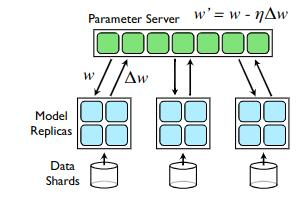
\includegraphics{Parts/images/Downpour_SGD.jpg}}
	\caption{Визуализация Downpour SGD}
	\label{framework} %framework,fig1
\end{figure}

\indent\setlength{\parindent}{1em} 
Преимуществом Downpour SGD по сравнению с синхронной распределенной вариацией SGD является его устойчивость к отказам машин, поскольку каждая реплика индивидуально выполняет свою работу и по завершении не ждет остальных, чтобы обновить значения параметров. Основной проблемой асинхронного подхода является невозможность поддержания консистентности значений параметров для каждой реплики. Поскольку каждая реплика действует независимо, то нет никакой гарантии, что в любой момент времени к параметрам на разных машинах было применено одинаковое количество обновлений или что обновления были применены в одном и том же порядке.

\subsection{Sandblaster L-BFGS}
\indent\setlength{\parindent}{1em} 
Авторы рассматривают распределенное обучение модели L-BFGS, заключающееся в параллелизме данных.  

\indent\setlength{\parindent}{1em} 
Ключевые идеи распределенности для алгоритма L-BFGS, которые предлагают авторы статьи:
\begin{itemize}
  \item распределенное хранение параметров 
  \item выделение процесса координатора, который не имеет доступа к параметрам модели и выступает в роли оркестратора всех реплик, выполняющих обучение
\end{itemize}

\indent\setlength{\parindent}{1em} 
Координатор назначает каждой из реплик модели небольшую часть работы, которую она может выполнить независимо, и каждый раз, когда какая-то реплика заканчивает свою работу, координатор назначает ей новую часть. Такой подход позволяет хорошо использовать быстрые машины и исключает ожидания самой медленной реплики, чтобы продолжить процесс. Результаты работы, а также кэшируемая информация сохраняются локально на каждой реплике и не отсылаются в центральный сервер, что позволяет запускать обучение достаточно больших моделей без оверхеда на отправку и сбор всех параметров. 

\begin{figure}[h]%current location
	\centering
	\scalebox{0.4}{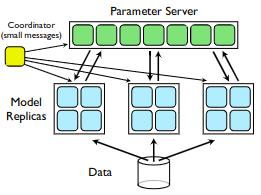
\includegraphics{Parts/images/Sandblaster_L-BFGS.jpg}}
	\caption{Визуализация Sandblaster L-BFGS}
	\label{framework} %framework,fig1
\end{figure}

\subsection{Достигнутые результаты и проверка эффективности}
\indent\setlength{\parindent}{1em} 
Авторы статьи применяют описанные методы оптимизации для двух задач глубинного обучения: распознавание объектов на изображениях и акустическая обработка для распознавания речи.
Ниже приведены графики для задачи обработки речи. Авторы сравнивают три оптимизационных модели, которые тренируются распределённо: Downpour SGD, Downpour SGD w Adagrad, Sandblaster L-BFGS с двумя моделями, которые были обучены на центральном процессоре одной реплики (черная линия) и на оптимизированном графическом процессоре (розовая пунктирная линия).
\begin{figure}[h]%current location
	\centering
	\scalebox{0.4}{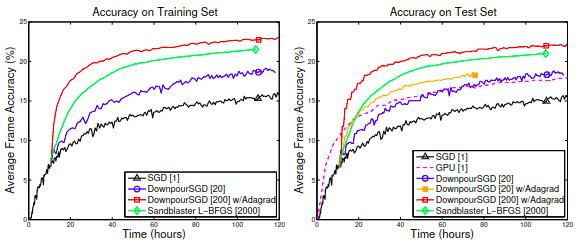
\includegraphics{Parts/images/time_accuracy.jpg}}
	\caption{Зависимость точности модели от времени обучения}
	\label{framework} %framework,fig1
\end{figure}

\indent\setlength{\parindent}{1em} 
Весьма значительным результатом является то, что авторы статьи применили разработанный метод оптимизации к модели с 1.7 миллиардами параметров и получили точность классификации 15\% на кросс валидации, что является относительным улучшением более чем на 60\% по сравнению с лучшей производительностью в этой задаче классификации.
